% PSS: A Cognitive Runtime Above Perception
% arXiv skeleton. Compile with pdflatex + bibtex (or upload the whole
% paper/ directory to arXiv/Overleaf). Replace TODO comments with the final
% text before submission.

\documentclass[11pt]{article}

\usepackage[T1]{fontenc}
\usepackage[utf8]{inputenc}
\usepackage{times}
\usepackage[margin=1in]{geometry}
\usepackage{amsmath,amssymb}
\usepackage{booktabs}
\usepackage{graphicx}
\usepackage{multirow}
\usepackage{array}
\usepackage{enumitem}
\usepackage{caption}
\usepackage{subcaption}
\usepackage{xcolor}
\usepackage{tikz}
\usetikzlibrary{positioning,arrows.meta}
\usepackage[numbers,round]{natbib}
\usepackage{url}
\usepackage[colorlinks=true,linkcolor=blue,citecolor=blue,urlcolor=blue]{hyperref}

\newcommand{\pss}{PSS}
\newcommand{\todo}[1]{\textcolor{red}{[TODO: #1]}}

\title{\pss: A Cognitive Runtime Above Perception\\[2pt]
\large Contract-Level Modularity and Property-Level Evaluation for Embodied AI}

\author{Jiahe Qi\\
Independent Researcher\\
ORCID: 0009-0001-8379-631X\\
\texttt{qijiaheX@126.com}\\
\small Code and reports: \url{https://github.com/Shirlif/PublicSemanticSpace}}

\date{}

\begin{document}

\maketitle

\begin{abstract}
Embodied systems keep upgrading their perception stack, but their cognitive
state---identity, relations, memory, and audit---usually lives inside an
end-to-end model. Swapping an expert then forces retraining the whole stack,
knowledge updates cannot be inspected or rolled back, and inference cost has no
hard bound. We present \pss, a cognitive runtime above perception: a pluggable
expert layer governed by an admission contract, a public semantic space used as
a calibratable interface rather than a zero-shot coordinate system, and an
explicit state layer that maintains persistent entity identity, typed relations,
active-set memory, a versioned truth-maintenance store, and bounded inference.
We evaluate \pss at the property level, treating expert quality as a controlled
factor, pairing architecture variants as twins, and testing the metrics with
negative controls. Across L0/L1 experiments the hot-swap contract (swap
success, rollback exactness, non-interference, routing) is invariant to expert
quality, while semantic compatibility is not: cross-family zero-shot swap falls
to chance, and one-shot calibration recovers vision but not tactile.
Entity-state audit, typed relations, active-set selection, and bounded
inference are measured separately, and an L2 bundle replay isolates the
contribution of the memory layer from the perception stream. We report boundary
conditions and negative results, including a $+0.012$ fair-attribution
re-identification gain and a case where retraining experts is no better than
rebuilding prototypes on frozen features. \pss is not a foundation model; it is
a contract-level runtime and a measurement protocol.
\end{abstract}

%-------------------------------------------------------------------------------
\section{Introduction}
\label{sec:intro}

Embodied systems are in a permanent upgrade cycle: encoders improve, modalities
are added, sensors are replaced. The perception stack is expected to change.
The cognitive state---who is who, what is related to what, what is remembered,
what can be rolled back---is usually buried in the same end-to-end model. This
creates three failures:

\begin{enumerate}[leftmargin=*]
  \item \textbf{No hot-swap.} Replacing one expert forces retraining or
        fine-tuning the whole stack; it is hard to show that only the intended
        module changed.
  \item \textbf{No knowledge transaction.} Facts, rules, and prototypes are
        updated by changing parameters or retraining, so locality, rollback,
        and audit are undefined.
  \item \textbf{No cost bound.} Inference grows with history or context, with
        no hard cap and no graceful degradation.
\end{enumerate}

Existing evaluations often mix these properties with end-to-end accuracy. A
higher score can come from a stronger encoder, a better-tuned projection, a
different prototype, or the architecture itself. Without a controlled
comparison, the architectural contribution is not identified.

\paragraph{This paper.}
\pss treats the cognitive state as a first-class, explicit layer above frozen
sensory experts. The public semantic space is an alignment interface between
experts and that layer, not a universal coordinate system. The architecture is
governed by four contracts: expert admission, hot-swap, versioned knowledge, and
bounded inference. The evaluation is property-level: expert quality is a
controlled factor, architecture variants are paired twins, and negative
controls test whether the metrics are sensitive.

\paragraph{Contributions.}
\begin{itemize}[leftmargin=*]
  \item \textbf{C1 (cognitive state).} An explicit entity layer with persistent
        identity, lifecycle, provenance, and auditable retraction/rollback; a
        property suite measures provenance completeness, retraction correctness,
        rollback exactness, and tamper detection.
  \item \textbf{C2 (typed relations).} Spatial, semantic, and tactile relation
        heads; exact geometric predicates remain the backbone, and learned
        relations act as a calibration channel only inside their training
        regime.
  \item \textbf{C3 (active-set memory).} Observation-conditioned selection
        matches full-candidate accuracy with a small number of candidates; the
        long-horizon fact-selection failure is traced to a missing
        query-conditioning interface.
  \item \textbf{C4 (contract preconditions).} Admission, atomic hot-swap,
        versioned knowledge with TMS justifications, and bounded inference are
        measured independently of expert quality; a contract-free baseline
        fails the same suite.
  \item \textbf{C5 (evaluation protocol).} A property-level protocol with
        expert-quality control, twin pairing, negative controls, equivalence
        tests, variance decomposition, and preregistration.
  \item \textbf{C6 (calibratable interface).} Cross-family zero-shot swap is
        not assumed; calibration is part of admission, and its cost is reported
        separately from capability.
\end{itemize}

\paragraph{What this paper is not.}
It does not claim state-of-the-art perception, zero-shot semantic compatibility
across expert families, real-robot reliability, or large-scale scaling. It is a
systems and measurement paper.

%-------------------------------------------------------------------------------
\section{Related Work}
\label{sec:related}

\paragraph{Modular deep learning.}
Adapters, mixture-of-experts, and model merging study how to train and combine
modules \citep{pfeiffer2023modular}. \pss focuses on what happens \emph{after} a
module is swapped: admission, routing, non-interference, rollback, and audit.

\paragraph{Knowledge update and truth maintenance.}
Knowledge editing and retrieval-augmented models update or retrieve facts
\citep{lewis2020rag,meng2022rome,decao2021editing}. Truth-maintenance systems
maintain justifications and propagate retractions \citep{doyle1979tms}. \pss
puts a TMS-style layer behind the production fact store and measures atomicity,
locality, propagation, conflict detection, rollback, and audit.

\paragraph{Bounded inference.}
Anytime and resource-bounded reasoning trade quality for a hard budget
\citep{zilberstein1996anytime}. \pss makes the budget a runtime contract:
entity, relation, expansion, and latency caps, with an explicit degradation
FSM.

\paragraph{Cognitive architectures and world models.}
Cognitive architectures organize perception, memory, and action
\citep{eliasmith2012spaun,sumers2024coala}; world models learn dynamics for
planning \citep{hafner2023dreamerv3,bardes2024vjepa}. \pss does not compete with
a learned world model; it makes the state between perception and action explicit
and auditable.

%-------------------------------------------------------------------------------
\section{\pss: Architecture and Contracts}
\label{sec:method}

\subsection{Overview}

\begin{figure}[t]
\centering
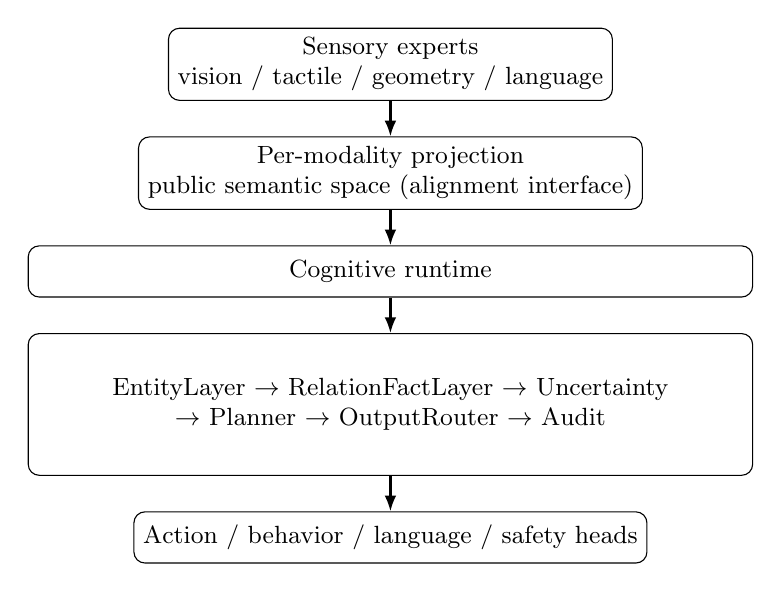
\begin{tikzpicture}[
  node distance=4.5mm and 6mm,
  box/.style={draw, rounded corners, align=center, minimum width=5.2cm,
              minimum height=0.65cm, font=\small},
  wide/.style={box, minimum width=9.2cm},
  arrow/.style={-{Latex[length=2mm]}, thick}
]
\node[box] (experts) {Sensory experts\\vision / tactile / geometry / language};
\node[box, below=of experts] (proj) {Per-modality projection\\public semantic space (alignment interface)};
\node[wide, below=of proj] (runtime) {Cognitive runtime};
\node[wide, below=of runtime, minimum height=1.8cm] (layers)
  {EntityLayer $\rightarrow$ RelationFactLayer $\rightarrow$ Uncertainty\\
   $\rightarrow$ Planner $\rightarrow$ OutputRouter $\rightarrow$ Audit};
\node[box, below=of layers] (out) {Action / behavior / language / safety heads};
\draw[arrow] (experts) -- (proj);
\draw[arrow] (proj) -- (runtime);
\draw[arrow] (runtime) -- (layers);
\draw[arrow] (layers) -- (out);
\end{tikzpicture}
\caption{\pss sits above perception. Experts are frozen or slowly updated; the
public semantic space is a per-modality alignment interface; the cognitive
runtime maintains explicit state, knowledge, uncertainty, plans, and audit.}
\label{fig:architecture}
\end{figure}

Figure~\ref{fig:architecture} shows the layering. \pss does not encode images or
text; it binds observations into persistent entities, computes typed relations,
maintains active-set memory and versioned facts, plans under a budget, and
routes the state to action, language, or safety heads.

\subsection{Expert contract and hot-swap}

An expert declares its modality, version, output dimension, encoder, and health.
The admission contract validates these fields, probes the expert on a fixed
batch, and rejects invalid modules. A swap is atomic: the old module remains
active on failure, the new module is routed by modality and version, unrelated
modules are behavior-hashed before and after, and rollback restores the previous
module exactly.

\subsection{Public semantic space as a calibratable interface}

Each modality has its own projection and prototype bank. We never sum
modalities into a single vector: addition is not separable, and the per-modality
structure is what allows cross-modal retrieval. The space is not assumed to be
shared zero-shot across expert families. A new family is admitted with a small
calibration set; the calibration cost is reported as part of the swap, not hidden
in an end-to-end score.

\subsection{Explicit cognitive state}

The runtime maintains:
\begin{itemize}[leftmargin=*]
  \item persistent entity IDs, lifecycle, attributes, confidence, and provenance;
  \item typed relation facts (spatial, semantic, tactile) written into a scene
        graph;
  \item active-set memory and versioned facts with TMS justifications;
  \item uncertainty, conflict, abstention, and an audit log;
  \item snapshots, rollback, and permission-scoped actions.
\end{itemize}
Entity state changes carry provenance; retraction removes only the target
attribute; rollback restores a bit-exact state hash; an edited audit entry is
detected by a hash chain.

\subsection{Bounded inference}

The budget controller caps the number of entities, relations, planner
expansions, and retrieval levels. The planner is anytime: it returns a valid
partial plan at interruption, and a degradation FSM moves between normal,
warning, degraded, emergency, and offline states. Budget adherence, monotonicity,
and degradation correctness are measured as properties.

\subsection{Property versus capability}

\begin{table}[t]
\centering
\small
\begin{tabular}{@{}p{0.22\linewidth}p{0.34\linewidth}p{0.34\linewidth}@{}}
\toprule
 & \textbf{Property} & \textbf{Capability} \\
\midrule
Examples & SSR, RBE, INT, RCR, LOC, PCR, AUD, BAR & ZCR, accuracy, re-ID, task success \\
Expert-quality dependence & should be flat & varies with expert quality \\
Purpose & architecture contract & expert/interface diagnostics \\
\bottomrule
\end{tabular}
\caption{Property metrics are designed to be invariant to expert quality;
capability metrics are not. Mixing them is the confound this paper avoids.}
\label{tab:property-capability}
\end{table}

Table~\ref{tab:property-capability} is the pivot of the evaluation. If a metric
moves with expert quality, it is a capability or diagnostic, not a contract
property. ZCR is treated as capability for this reason.

%-------------------------------------------------------------------------------
\section{Evaluation Protocol}
\label{sec:evaluation}

\paragraph{Levels.}
\textbf{L0} uses structured observations and expert stubs to isolate the
architecture. \textbf{L1} uses real frozen experts, projections, and
prototypes. \textbf{L2} uses bundle replay and a fresh Isaac S4-PSS episode for
external validity. Primary evidence is L0/L1; L2 can reveal contract violations
but does not overturn a property claim.

\paragraph{Factors.}
Expert quality $Q0$ (oracle) through $Q4$ (random) is a controlled factor.
Architecture variants include full, per-modality, flat KB, unbounded, naive
swap, and retrain-all (oracle upper bound). Difficulty is varied separately.

\paragraph{Pairing.}
Each treated run has a control twin with the same spec hash, seed, scene, and
episode; only the architecture or operation differs. Paired differences are the
unit of causal analysis.

\paragraph{Negative controls.}
N1--N8 deliberately break one contract at a time: flat KB, unbounded planner,
naive swap, random expert, shuffled embeddings, no-op update, and an
over-budget controller. A control that does not fail as specified invalidates
the suite.

\paragraph{Statistics and preregistration.}
We report paired bootstrap confidence intervals, TOST equivalence tests for
invariance, and two-way ANOVA for descriptive variance decomposition. Metrics,
thresholds, and kill criteria are frozen in
\texttt{eval/property\_preregistration.md}; deviations are recorded and labelled
exploratory.

%-------------------------------------------------------------------------------
\section{Results}
\label{sec:results}

All numbers below are from the public scorecards and claim-gap reports in the
repository. We separate what is supported from what is not.

\subsection{Contract invariance}

\begin{table}[t]
\centering
\small
\begin{tabular}{@{}lccccc@{}}
\toprule
Metric & Q0 & Q1 & Q2 & Q3 & Q4 \\
\midrule
SSR & 1.000 & 1.000 & 1.000 & 1.000 & 1.000 \\
ZCR & 0.969 & 0.878 & 0.757 & 0.587 & 0.142 \\
INT & 0.000 & 0.000 & 0.000 & 0.000 & 0.000 \\
RBE & 1.000 & 1.000 & 1.000 & 1.000 & 1.000 \\
\bottomrule
\end{tabular}
\caption{L0 contract metrics across expert quality (5 seeds). SSR, INT, and RBE
are flat; ZCR tracks expert quality and is therefore a capability metric.}
\label{tab:contract}
\end{table}

Table~\ref{tab:contract} is the central contract result: swap success,
interference, and rollback exactness do not move as the expert degrades. ZCR
does move, which is why it is reported separately.

\begin{figure}[t]
\centering
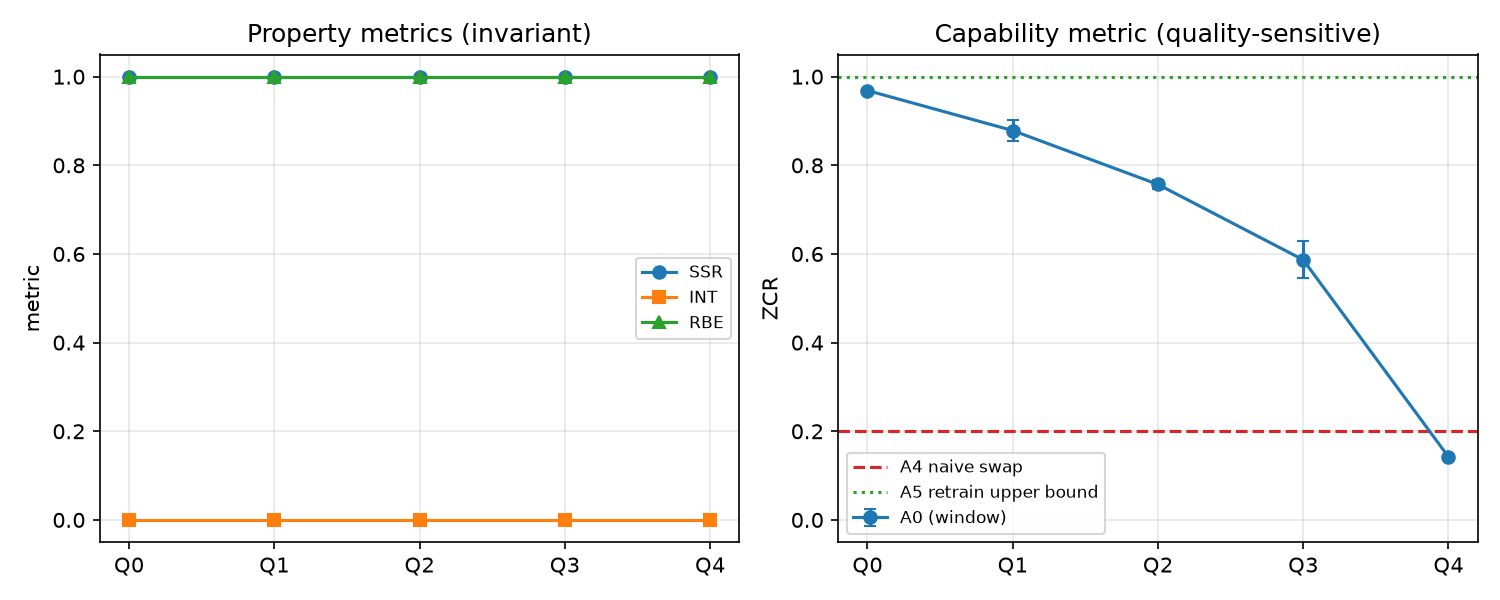
\includegraphics[width=0.92\linewidth]{figures/fig1_invariance.png}
\caption{Invariance plot. Left: SSR, INT, and RBE stay flat across expert
quality. Right: ZCR declines, confirming that it is a capability metric.}
\label{fig:invariance}
\end{figure}

\subsection{Cognitive state and binding}

\begin{table}[t]
\centering
\small
\begin{tabular}{@{}lccc@{}}
\toprule
Variant & ID retention & Switches & Reappearance \\
\midrule
graph + tactile & 0.989 & 0.02 & 0.978 \\
tactile zeroed & 0.872 & 0.26 & 0.744 \\
vision zeroed & 0.961 & 0.08 & 0.922 \\
simple tracker & 0.917 & 0.17 & 0.833 \\
text-state proxy & 0.500 & 1.00 & 0.000 \\
\bottomrule
\end{tabular}
\caption{Binding under a 70-frame full occlusion (60 sequences $\times$ 3 seeds).
Same tracker, only the input channel is ablated. Contribution: tactile
$+0.117$, graph/state $+0.072$, vision $+0.028$, state over no memory $+0.489$.}
\label{tab:binding}
\end{table}

Entity-state audit (E1) reports provenance completeness, retraction correctness,
rebind identity, rollback exactness, and tamper detection all at $1.00$; the
three negative controls (no audit log, no hash chain, shallow snapshot) fail
their targeted metric at $0.00$. Binding is strong (Table~\ref{tab:binding}),
but the decomposition shows that most of the signal is tactile, not the graph
layer. The fair-attribution re-ID gain over a transformer is only $+0.012$.

\begin{figure}[t]
\centering
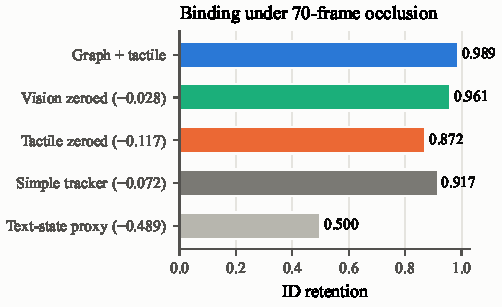
\includegraphics[width=0.9\linewidth]{figures/fig_binding_signal.pdf}
\caption{Binding under a 70-frame occlusion (E2). The same tracker is run with
one input channel ablated; deltas are relative to graph+tactile. Tactile is the
largest sensory contributor, but the state layer supplies most of the gain over
the no-memory proxy.}
\label{fig:binding}
\end{figure}

\begin{figure}[t]
\centering
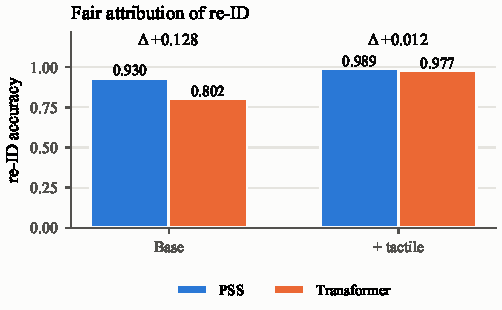
\includegraphics[width=0.82\linewidth]{figures/fig_fair_attribution.pdf}
\caption{Fair attribution of re-ID. Without tactile, \pss is $+0.128$ over the
transformer; with the same tactile input, the gain is $+0.012$. The protocol
reduces the architectural claim rather than inflating it.}
\label{fig:fair}
\end{figure}

\subsection{Typed relations}

\begin{table}[t]
\centering
\small
\begin{tabular}{@{}lcc@{}}
\toprule
Relation type & F1 (clean) & F1 (tactile removed) \\
\midrule
spatial & 0.957 & -- \\
semantic & 0.996 & -- \\
tactile & 0.970 & 0.483 \\
\bottomrule
\end{tabular}
\caption{Typed relation heads. Removing tactile drops tactile F1 to 0.483,
which shows the head is not using a shortcut.}
\label{tab:relations}
\end{table}

\begin{table}[t]
\centering
\small
\begin{tabular}{@{}lc@{}}
\toprule
Method & Exact-4 accuracy at noise 0.15 \\
\midrule
geometry ($\epsilon=0.1$) & 0.537 \\
geometry (dead zone 0.25) & 0.828 \\
learned & 0.532 \\
naive hybrid & 0.503 \\
distribution-aware hybrid & 0.857 \\
\bottomrule
\end{tabular}
\caption{Hybrid relations under coordinate noise on held-out regions. Learned
relations help only inside their training regime; applying them to unseen
aligned axes is worse than geometry.}
\label{tab:hybrid}
\end{table}

The correct form is a hybrid: exact geometry owns aligned and held-out axes,
learned relations calibrate the clear-diagonal regime. Pure learned relations do
not replace geometry.

\begin{figure}[t]
\centering
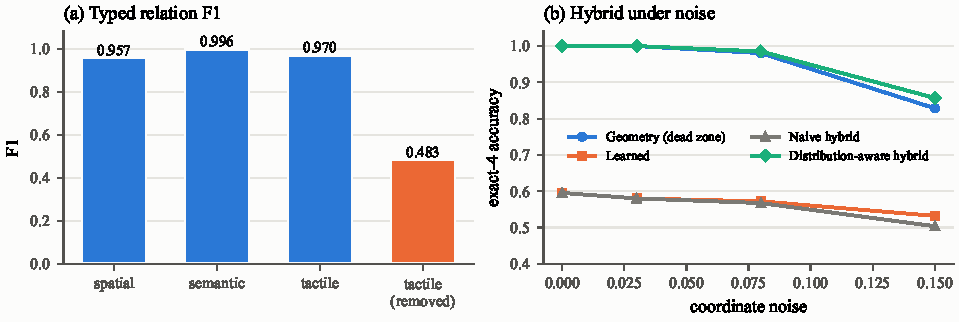
\includegraphics[width=\linewidth]{figures/fig_relations.pdf}
\caption{(a) Typed relation F1; removing tactile drops tactile F1 to 0.483.
(b) Hybrid relations under coordinate noise on held-out regions. Learned
relations help only inside their training regime; the naive hybrid is worse
than geometry.}
\label{fig:relations}
\end{figure}

\subsection{Memory and bounded inference}

\begin{table}[t]
\centering
\small
\begin{tabular}{@{}p{0.44\linewidth}p{0.46\linewidth}@{}}
\toprule
Setting & Result \\
\midrule
re-ID candidates, $k=1$ + fallback & 0.972 $\rightarrow$ 1.000, $\sim$1.2 candidates \\
compute, $N=200$ / $N=1000$ & 6.4$\times$ / 23.6$\times$ \\
long-history fact, $k=4$: hot / old learned / query-conditioned & 0.237 / 0.241 / 1.000 \\
exact-RAG vs \pss latency & 1.38 ms vs 0.0003 ms \\
\bottomrule
\end{tabular}
\caption{Active-set memory and bounded inference. The long-history negative
result is explained by query-independent scoring; a simple query-recency rule
matches the learned policy.}
\label{tab:memory}
\end{table}

The active-set advantage is a cost advantage, not a capability claim. Exact-RAG
with oracle retrieval reaches 1.000 accuracy but still scans the full history;
\pss performs a constant-time lookup over a small active set.

\begin{figure}[t]
\centering
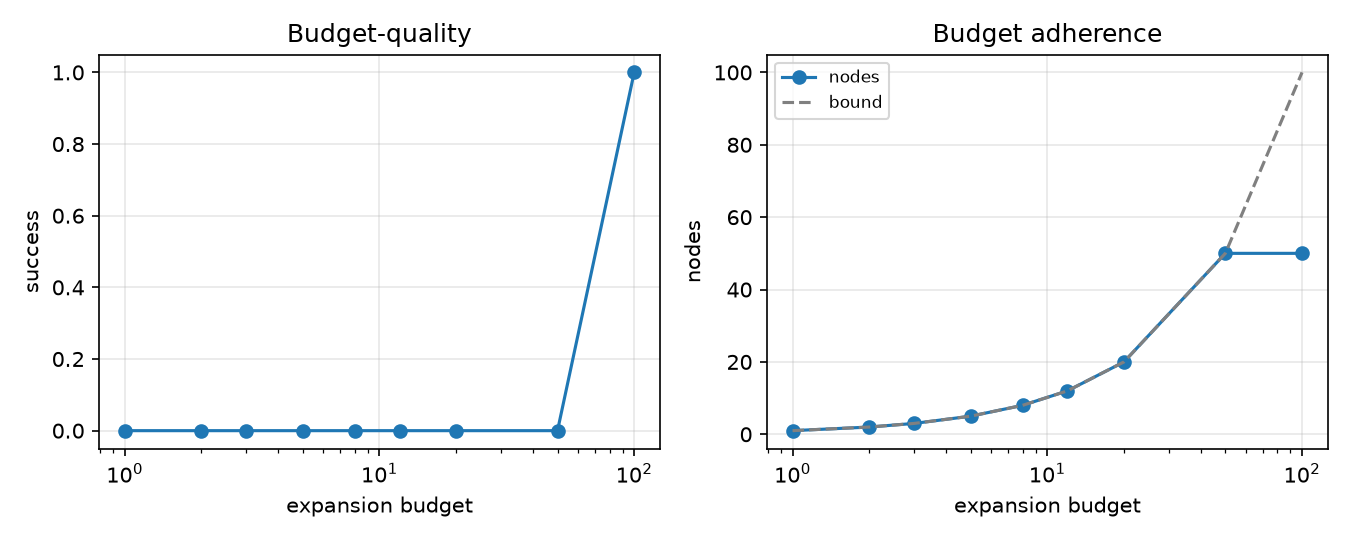
\includegraphics[width=0.9\linewidth]{figures/fig3_budget_quality.png}
\caption{Quality versus budget. The planner is anytime: quality is monotone in
the budget, and the budget controller keeps the node count within the cap.}
\label{fig:budget}
\end{figure}

\begin{figure}[t]
\centering
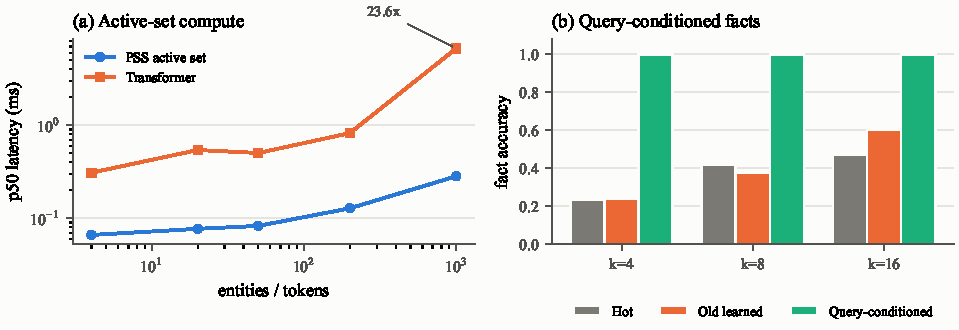
\includegraphics[width=\linewidth]{figures/fig_memory_compute.pdf}
\caption{(a) Active-set p50 latency vs entities/tokens (log-log). (b) Fact
accuracy at $k=4/8/16$; query conditioning recovers full accuracy, and a simple
recency rule matches the learned policy.}
\label{fig:memory}
\end{figure}

\subsection{Knowledge updates and TMS}

K1--K8 exercise assert, retract, locality, dependency propagation, conflict
detection, rollback, adversarial updates, and multi-source priority. The
production \texttt{MultiSourceFactStore} is wrapped by
\texttt{TMSFactStore}; K3/K4/K5, audit completeness, and source retraction are
all $1.00$. Runtime permissions are also audited: \texttt{read\_only} denies
five actions, \texttt{admin} denies none, and denied actions appear in the audit
log.

\begin{figure}[t]
\centering
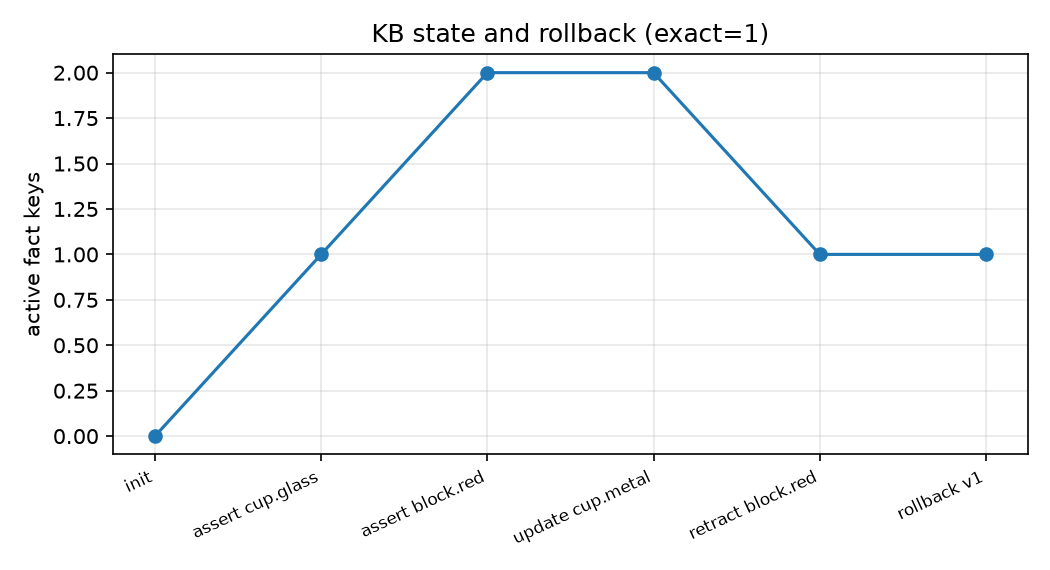
\includegraphics[width=0.9\linewidth]{figures/fig2_kb_state.png}
\caption{Knowledge-base state and rollback. A rollback restores the business
state hash exactly; the audit log records the change.}
\label{fig:kb}
\end{figure}

\subsection{Cross-family calibration and retraining cost}

\begin{table}[t]
\centering
\small
\begin{tabular}{@{}lccc@{}}
\toprule
Expert family & Vision zero-shot & Tactile zero-shot & Vision $k=1$ \\
\midrule
\texttt{category\_pretrain} & 0.200 & 0.067 & 1.000 \\
\texttt{category\_pretrain\_instance} & 0.167 & 0.067 & 0.900 \\
\texttt{category\_pretrain\_instance8} & 0.192 & 0.100 & 0.908 \\
\bottomrule
\end{tabular}
\caption{Cross-family swap and one-shot calibration (chance 0.167). The public
space is a calibratable interface, not a zero-shot coordinate system.}
\label{tab:families}
\end{table}

\begin{table}[t]
\centering
\small
\begin{tabular}{@{}lcc@{}}
\toprule
Method & Vision ZCR & Cost \\
\midrule
frozen expert + prototype rebuild & 0.964 & 3.2 ms \\
projection retrain & 0.979 & 13.5 s \\
30-epoch expert retrain + projection & 0.969 & 38 s \\
\bottomrule
\end{tabular}
\caption{Retraining cost. Rebuilding prototypes is the cheap step; retraining
experts is slower and does not improve accuracy.}
\label{tab:retrain}
\end{table}

Calibration is part of admission. The retraining experiment shows that a full
expert retrain is not necessary: prototype rebuild recovers most of the gap, and
projection retraining adds a small gain.

\begin{figure}[t]
\centering
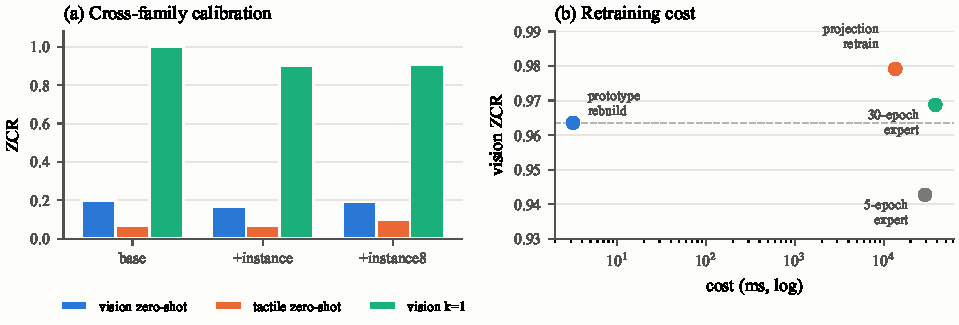
\includegraphics[width=\linewidth]{figures/fig_families_retrain.pdf}
\caption{(a) Cross-family zero-shot and one-shot vision calibration. (b) Vision
ZCR vs retraining cost on a log scale; prototype rebuild is the cheap step, and
expert retraining does not improve accuracy.}
\label{fig:families}
\end{figure}

\subsection{L2 external validity}

\begin{table}[t]
\centering
\small
\begin{tabular}{@{}lcc@{}}
\toprule
Bundle replay variant & ID retention & Switches \\
\midrule
full & 1.000 & 0.00 \\
\texttt{no\_memory} & 0.827 & 0.56 \\
\texttt{no\_entity} & 0.270 & 47.47 \\
\bottomrule
\end{tabular}
\caption{L2 bundle replay on the same detection stream (valid 19/33 bundles).
The state-layer ablation, not perception, explains the difference.}
\label{tab:l2-bundles}
\end{table}

\begin{table}[t]
\centering
\small
\begin{tabular}{@{}lc@{}}
\toprule
S4-PSS variant & Success \\
\midrule
full & 3/3 \\
\texttt{no\_memory} & 3/3 \\
\texttt{no\_entity} & 3/3 \\
\texttt{no\_relations} & 0/3 \\
\bottomrule
\end{tabular}
\caption{S4-PSS cognitive variants. This demo exercises relations, not memory;
the memory evidence is in Table~\ref{tab:l2-bundles}.}
\label{tab:s4}
\end{table}

\begin{figure}[t]
\centering
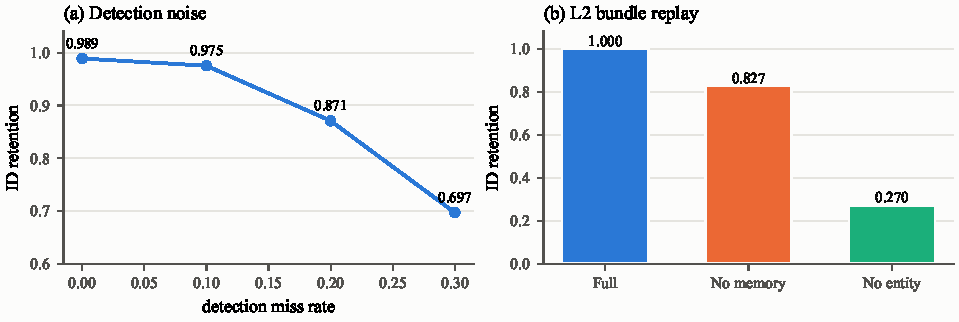
\includegraphics[width=\linewidth]{figures/fig_detection_l2.pdf}
\caption{(a) Binding under detection miss rate. (b) L2 bundle replay on the same
detection stream (valid 19/33 bundles); the state-layer ablation explains the
difference, not perception.}
\label{fig:detection-l2}
\end{figure}

\subsection{Semantic space and retrieval}

\begin{figure}[t]
\centering
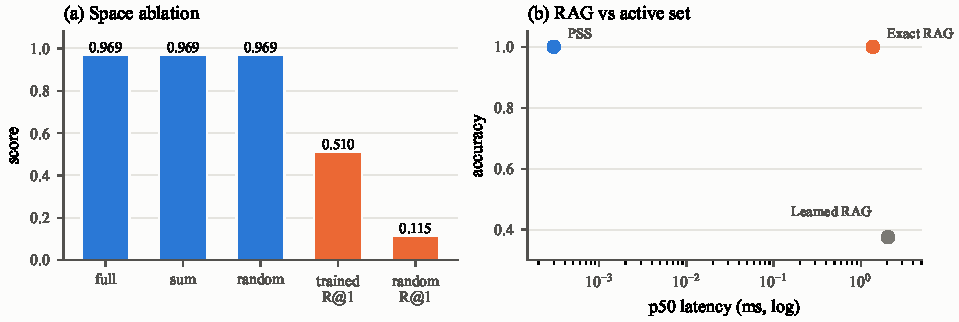
\includegraphics[width=\linewidth]{figures/fig_space_rag.pdf}
\caption{(a) Closed-set accuracy is invariant across the full, summed, and
random-projection spaces; the learned projection's value is cross-modal R@1
(0.510 vs 0.115). (b) Exact RAG matches accuracy but scans the full history;
the \pss active set is a constant-time lookup.}
\label{fig:space-rag}
\end{figure}

The space ablation is a caution against claiming that per-modality projection
improves closed-set accuracy. It does not, because the prototype bank is re-fit
in each space. What it buys is cross-modal alignment. Similarly, the active-set
advantage is a cost advantage: exact-RAG reaches the same accuracy but scans the
full history, while \pss looks up a small active set.

\subsection{Modality conflict and open-set rejection}

\begin{figure}[t]
\centering
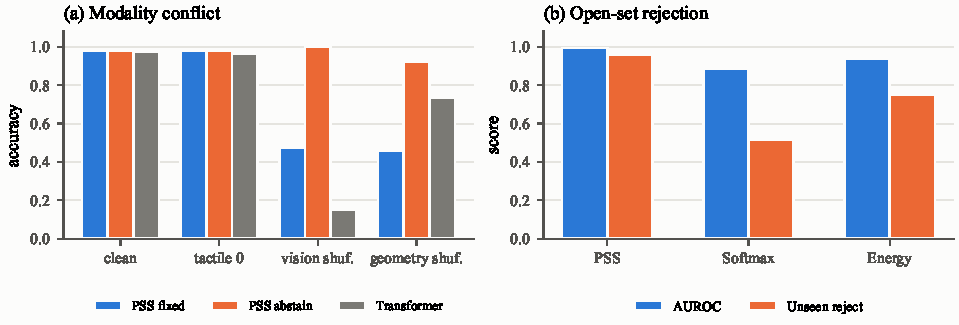
\includegraphics[width=\linewidth]{figures/fig_conflict_openset.pdf}
\caption{(a) Modality conflict: \pss fixed fusion vs abstention vs the
transformer. Under a shuffled vision channel, abstention keeps accepted accuracy
at 1.000 with coverage 0.083; the transformer has no explicit abstention.
(b) Open-set AUROC and unseen rejection.}
\label{fig:conflict-openset}
\end{figure}

The conflict experiment shows the intended behavior: when modalities disagree,
\pss can lower coverage and preserve accepted accuracy, rather than forcing a
prediction. The open-set result is a diagnostic of the prototype store, not a
property of the hot-swap contract.

\subsection{Negative controls}

\begin{table}[t]
\centering
\small
\begin{tabular}{@{}llll@{}}
\toprule
ID & Control & Expected & Observed \\
\midrule
N1 & flat KB & fail & LOC $>0$ / RBE $<1$ \\
N2 & unbounded planner & fail & BAR $<1$ \\
N3 & no admission validation & fail & invalid module accepted \\
N4 & random expert (capability) & fail & 0.21 \\
N5 & random expert (property) & pass & contract holds \\
N6 & no-op update & identity & hash equal \\
N7 & shuffled embeddings & capability fail, property pass & 0.125; contract holds \\
N8 & over-budget controller & fail & violations detected \\
\bottomrule
\end{tabular}
\caption{Negative controls. A control that does not behave as specified
invalidates the suite.}
\label{tab:controls}
\end{table}

\subsection{Contract-free baseline}

A contract-free baseline (no admission validation, no rollback, no versioned
routing, no audit, no budget controller) fails nine of twelve contract metrics;
\pss passes all twelve. This is the sensitivity check that the suite is not
describing \pss by construction.

%-------------------------------------------------------------------------------
\section{Discussion}
\label{sec:discussion}

\paragraph{The shared space is a protocol, not a coordinate system.}
Cross-family zero-shot swap fails; one-shot calibration recovers vision but not
tactile. The honest reading is that the public space is a calibratable
interface. Calibration is an admission cost, not a failure.

\paragraph{The state layer is the contribution, not accuracy.}
Fair attribution reduces the re-ID gain to $+0.012$. The value of the explicit
state layer is inspectability, rollback, and composition, not a higher score.

\paragraph{Learned relations calibrate, they do not replace geometry.}
The hybrid result is conditional: learned relations help in the clear-diagonal
regime they were trained on, and hurt on unseen aligned axes. Exact geometry
remains the backbone.

\paragraph{Optimization is not always retraining.}
Rebuilding prototypes on frozen features is milliseconds; retraining experts is
tens of seconds and does not improve accuracy. The paper should not claim that
retrain-all is expensive; it should claim that it is unnecessary.

%-------------------------------------------------------------------------------
\section{Limitations}
\label{sec:limitations}

\begin{itemize}[leftmargin=*]
  \item No real robot; all evidence is from MuJoCo, Isaac, and offline bundles.
  \item L2 uses oracle boxes/poses; H/K (hot-swap, knowledge update) are not
        executed in the Isaac task. Bundle replay and runtime-level tests cover
        part of the gap, but a perception-driven L2 bundle is still needed.
  \item Only three same-width expert families are connected; DINOv2,
        SqueezeNet, and WT-MM are not.
  \item The factorial design is reduced; L1 has five seeds.
  \item TMS is wrapped around the production fact store but not migrated to
        every call site.
  \item We do not claim SOTA, zero-shot public space, real-world reliability, or
        large-scale scaling.
\end{itemize}

%-------------------------------------------------------------------------------
\section{Conclusion}
\label{sec:conclusion}

\pss is a cognitive runtime above perception, not a foundation model. It makes
sensory experts pluggable under a contract, makes the cognitive state explicit
and auditable, and measures architectural claims with a property-level protocol
that separates expert quality from architecture. The evidence supports
contract-level modularity, a calibratable interface view of shared semantic
spaces, and honest negative results; it does not support capability SOTA or
zero-shot public-space claims. The next steps are a perception-driven L2 harness,
more expert families, a real-robot demonstration, and a competitive non-\pss
baseline for the evaluation protocol.

%-------------------------------------------------------------------------------
\appendix
\section{Claim--Evidence Map}
\label{app:claims}

\begin{table}[h]
\centering
\small
\begin{tabular}{@{}p{0.20\linewidth}p{0.42\linewidth}p{0.20\linewidth}@{}}
\toprule
Claim & Evidence & Strength \\
\midrule
C1 state & audit 1.00; 70-frame 0.989 vs 0.500; L2 1.000/0.827/0.270 & medium--strong \\
C2 relations & F1 0.957/0.996/0.970; hybrid 0.857 vs 0.828 & medium \\
C3 memory & 1.2 candidates; 6.4$\times$/23.6$\times$; query 0.241$\rightarrow$1.000 & medium--strong \\
C4 contracts & SSR/RBE/INT/RCR invariant; contract-free 0/9; scale flat & strong \\
C5 protocol & N1--N8; twins; preregistration; contract-free baseline & strong \\
C6 interface & zero-shot 0.186; $k=1$ 0.936; tactile 0.067--0.100 & medium--strong \\
\bottomrule
\end{tabular}
\caption{Compact claim--evidence map. The full version is in the repository.}
\end{table}

\section{Reproducibility}
\label{app:repro}

The repository contains the property suites, claim-gap experiments, raw
scorecards, manifests, and preregistration. A minimal reproduction:

\begin{verbatim}
pip install -e ".[train,sim]"
python -m pytest tests/property
python scripts/run_claim_gaps.py --run
python scripts/run_claim_gaps_followups.py
\end{verbatim}

Full commands and per-experiment reports are in
\texttt{reports/claim\_gaps/INDEX.md}. Raw scorecards are in
\texttt{scorecards/property/} with expert and run manifests.

%-------------------------------------------------------------------------------
\bibliographystyle{plainnat}
\bibliography{refs}

\end{document}
